%\begin{flushleft}
\begin{center}

\chapter{\large PROJECT ANALYSIS}

\justifying
\section{\normalsize USE CASE MODEL WITH SCENARIOS}
\vspace*{2mm}
\hspace{5mm} A Use case diagram captures use case and actor interactions.There are two level of use case diagram one context  level and other is requirement level.\\

\justifying
\subsection{\small Use Case level 0}
\vspace*{2mm}
\hspace{5mm}Here is the use case model level 0\\
\begin{figure}[H]
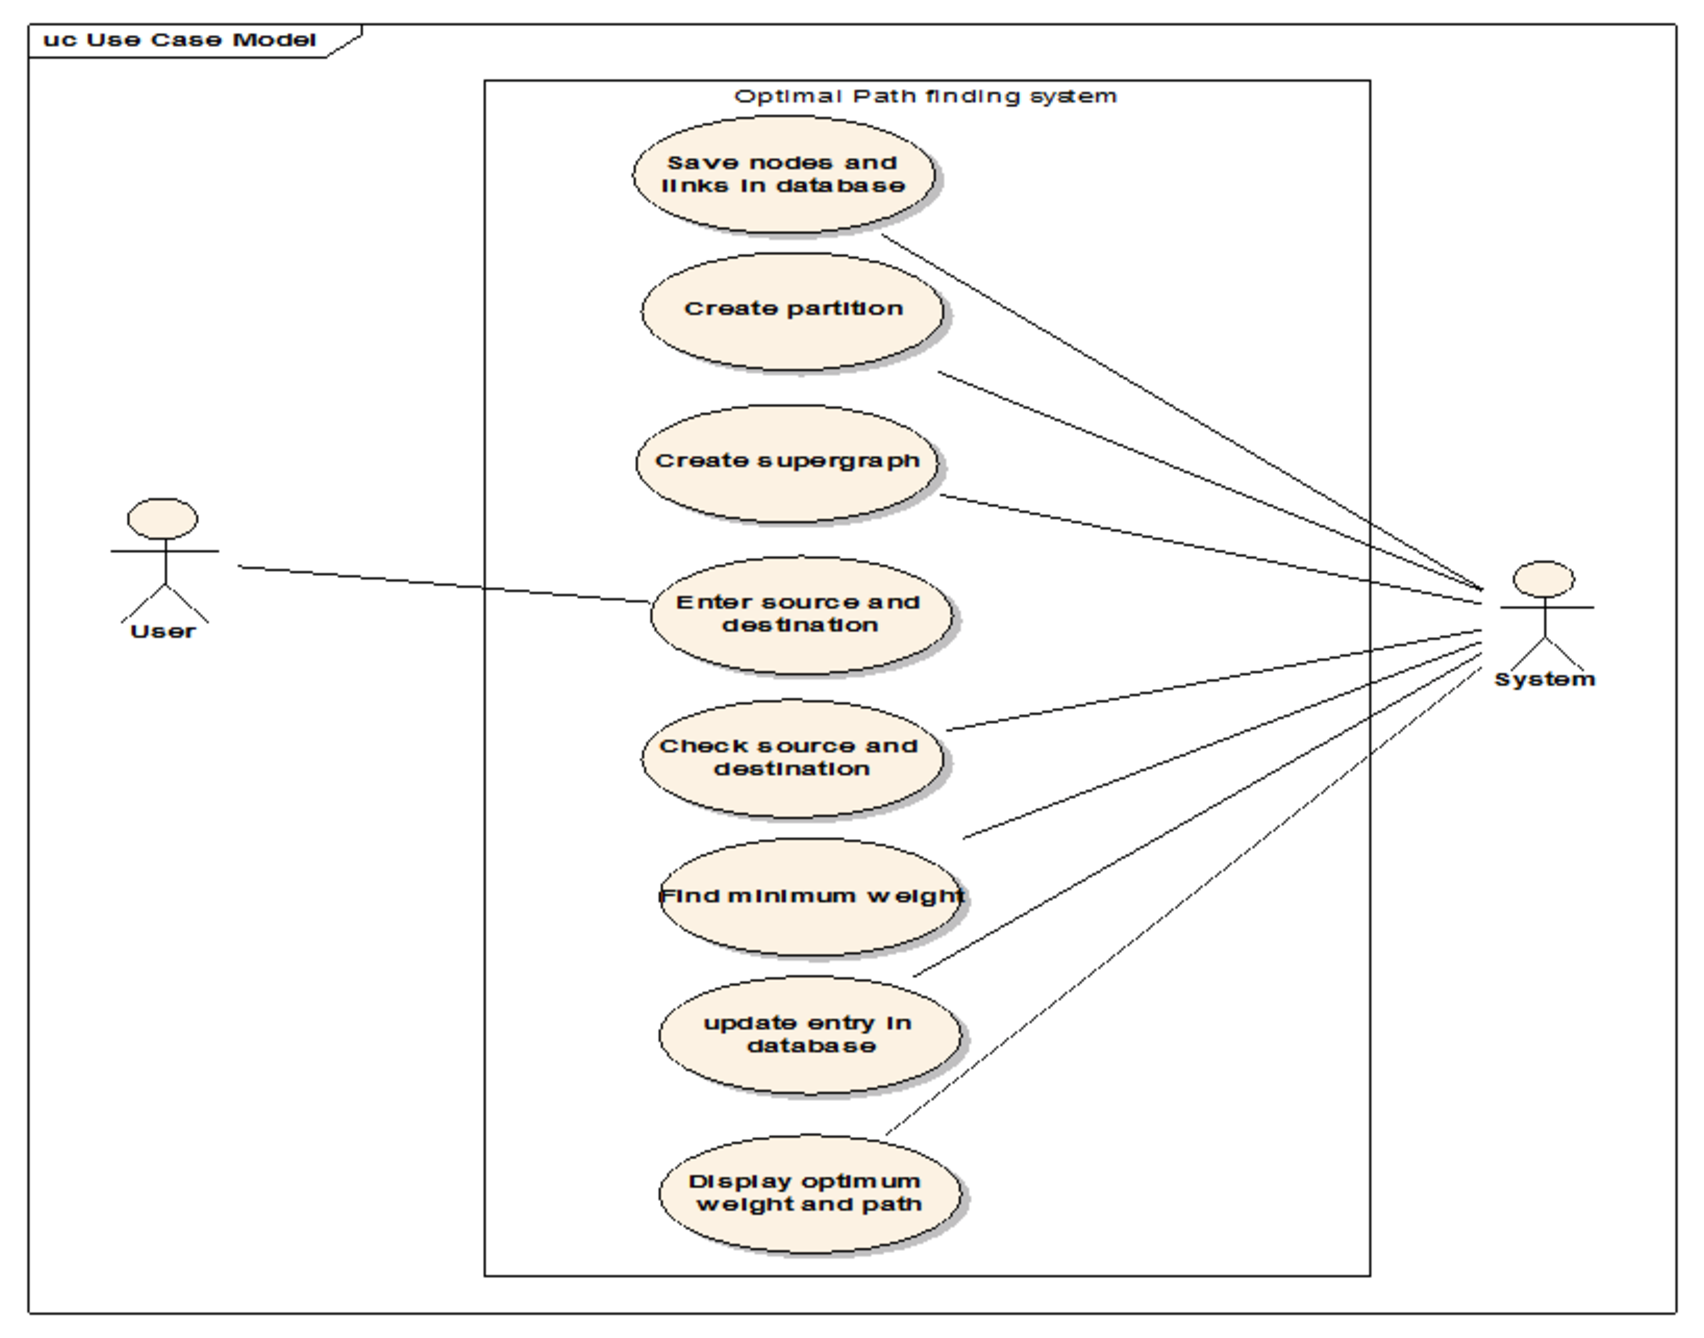
\includegraphics[width=13cm,height=8cm]{usecase0.eps}
\caption{Use Case Level 0}
\end{figure}
%\newpage


\subsection{\small Use Case level 1}
\begin{figure}[H]
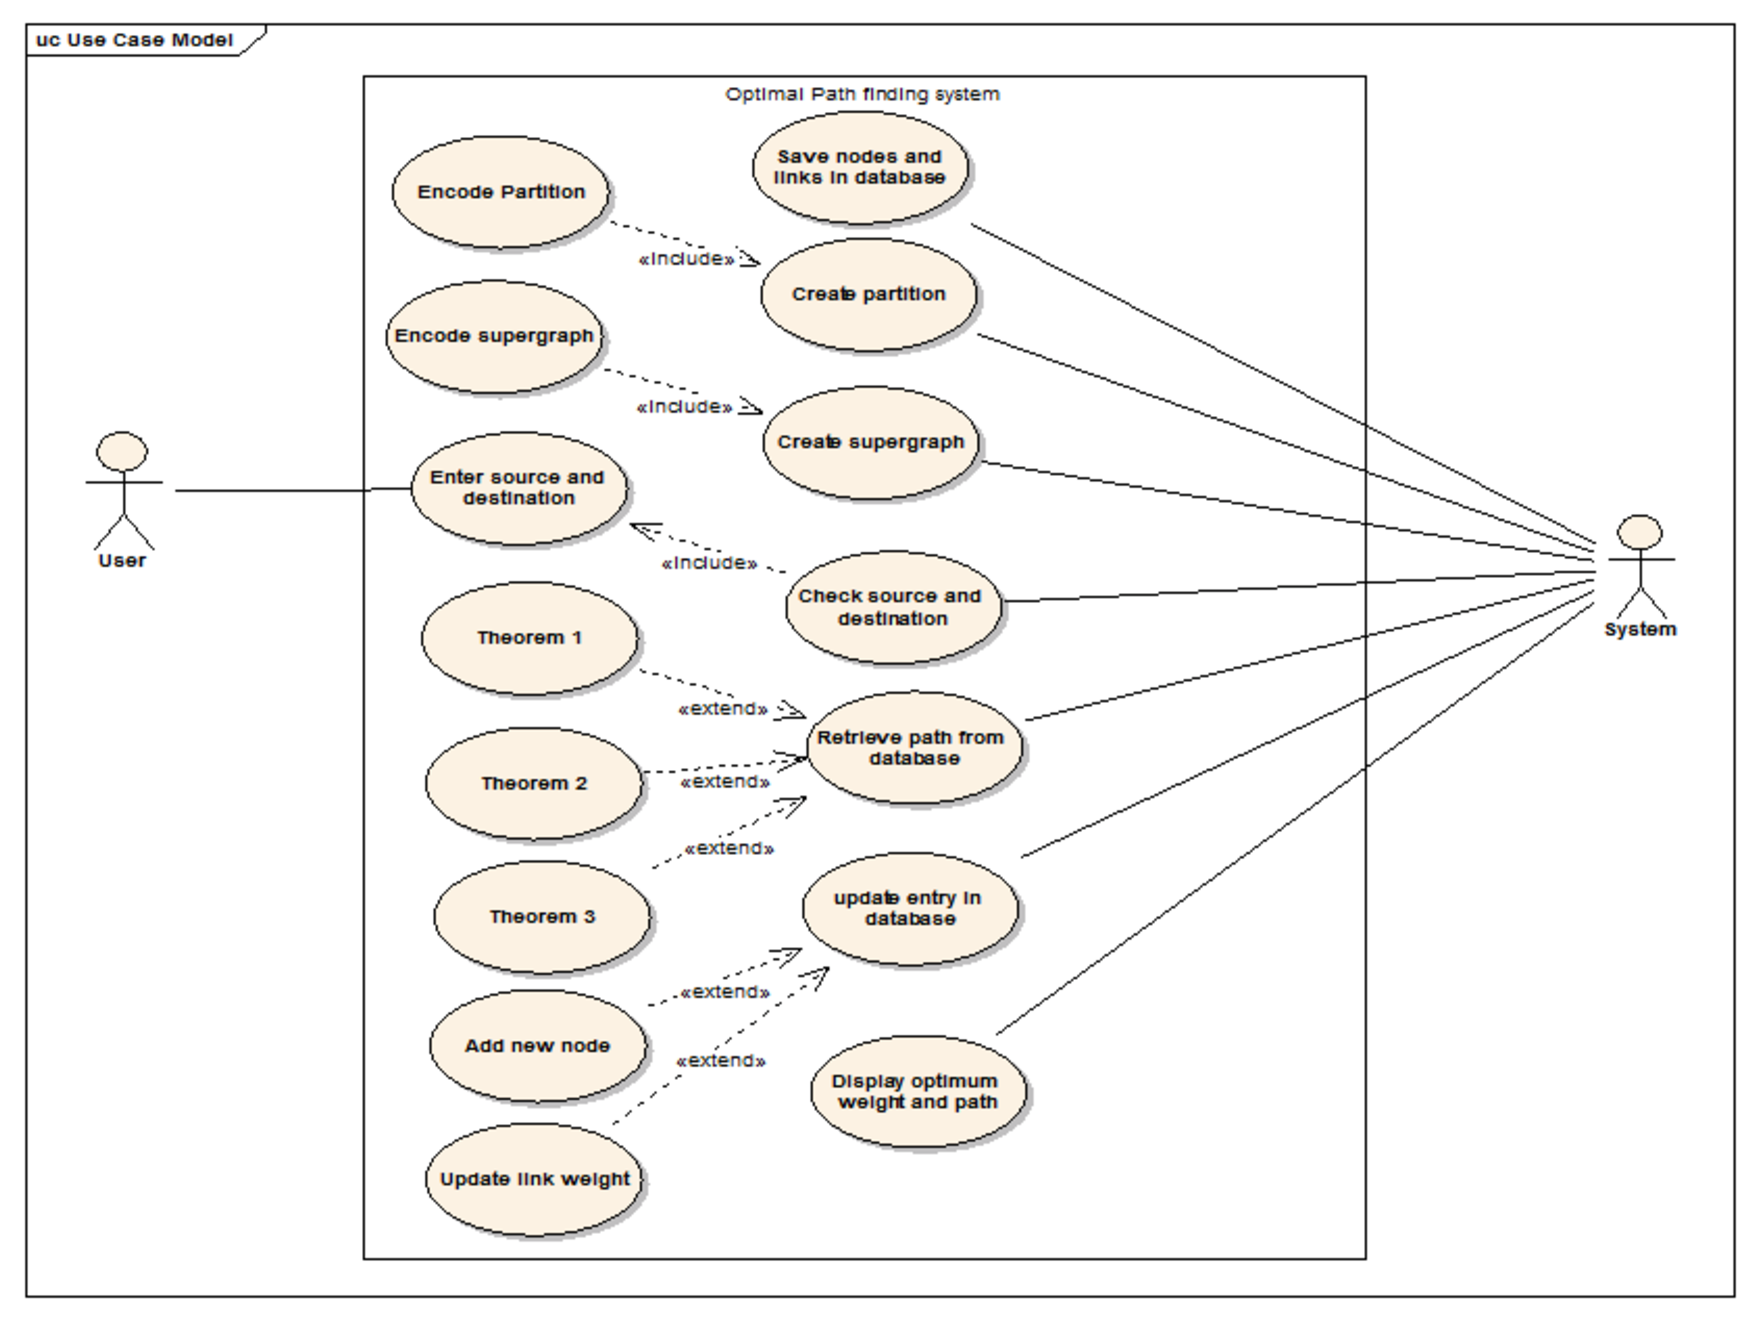
\includegraphics[width=15cm,height=16cm]{usecase1.eps}
\caption{Use Case level 1}
\end{figure}
\newpage

\section{\normalsize ACTIVITY DIAGRAM}
\hspace*{5mm}Activity diagrams are used to model the behaviours of a system, and the way in which these behaviours are related in an overall flow of the system. The logical paths a process follows, based on various conditions, concurrent processing, data access, interruptions and other logical path distinctions, are all used to construct a process, system or procedure.\\

\begin{figure}[H]
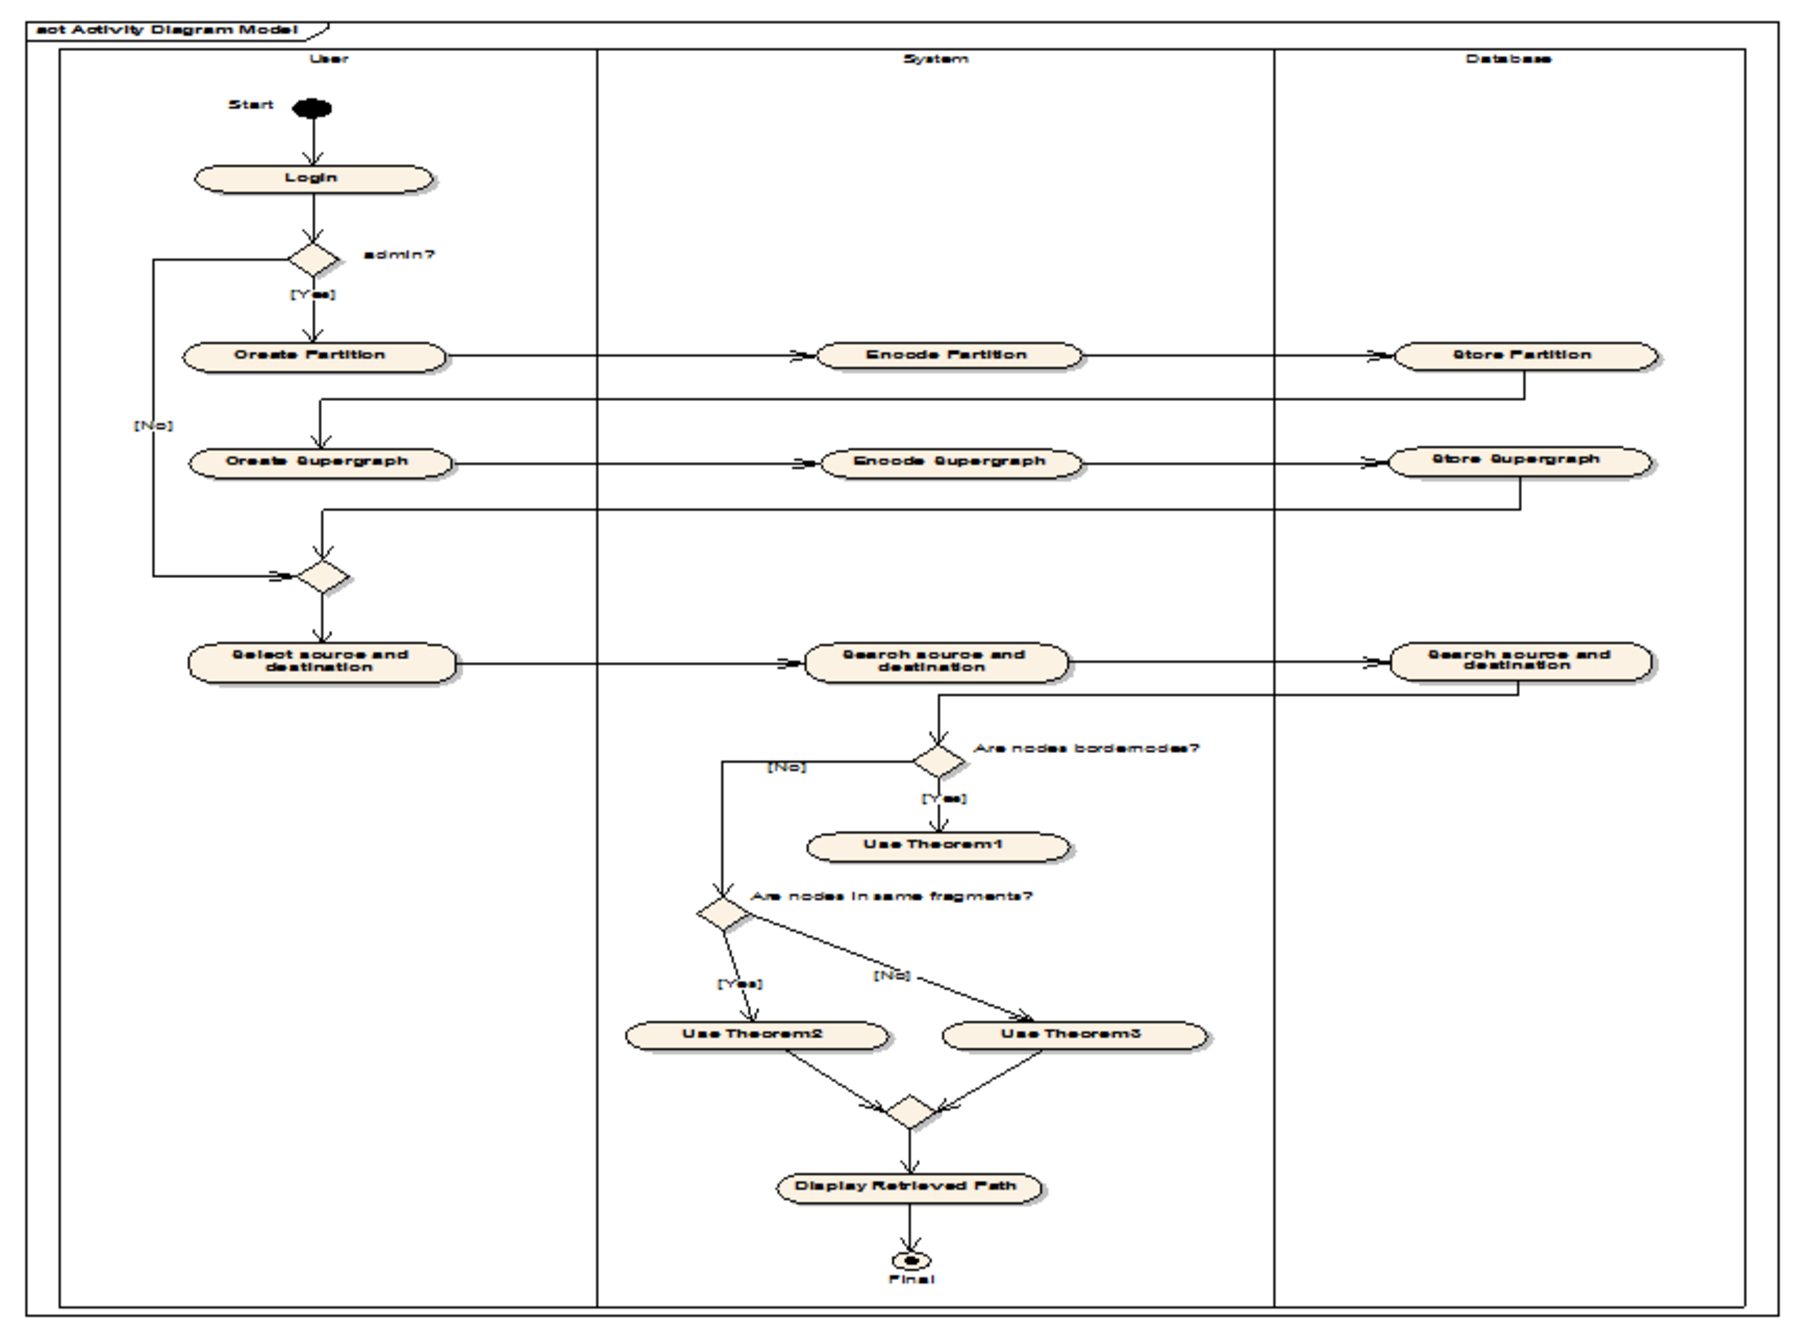
\includegraphics[width=16cm,height=13cm]{act.eps}
\caption{Activity Diagram}
\end{figure}
%\newpage
\end{center}
%\end{flushleft}